\section{Results}

\subsection{Sinus Regression}

All methods reduce the training and test loss on the sinus regression task. The final losses are very similar across methods, with best test losses between \(0.0716\) and \(0.0727\). Backpropagation reaches a best test loss of \(0.0717\), while IS-NP, vanilla NP, fan-in NP, and WP reach \(0.0727\), \(0.0717\), \(0.0716\), and \(0.0725\), respectively. The corresponding test \(R^2\) values are also close, ranging from \(0.553\) to \(0.559\). In terms of convergence speed, IS-NP reaches its convergence criterion earliest among the perturbation methods, at epoch \(73\), while WP is slowest, converging at epoch \(200\).

The estimator diagnostics show larger differences than the loss curves. The node perturbation methods have substantially higher cosine similarity than WP. IS-NP, fan-in NP, and vanilla NP obtain cosine similarities of \(0.812\), \(0.808\), and \(0.788\), respectively, while WP obtains \(0.524\). The same pattern appears in estimator variance. IS-NP, vanilla NP, and fan-in NP have variances of \(0.00649\), \(0.00717\), and \(0.00726\), respectively, whereas WP has a substantially larger variance of \(0.0555\).

For the sinus regression task, the differences in estimator quality are therefore much larger than the differences in final training and test performance. All methods are able to learn the task to a similar final loss, but the perturbation estimators differ clearly in directional alignment and variance. The node perturbation methods show better estimator diagnostics than WP, while IS-NP has the highest cosine similarity and the lowest variance among the perturbation-based methods.

\begin{figure}[!htbp]
    \centering
    \begin{subfigure}{0.95\textwidth}
        \centering
        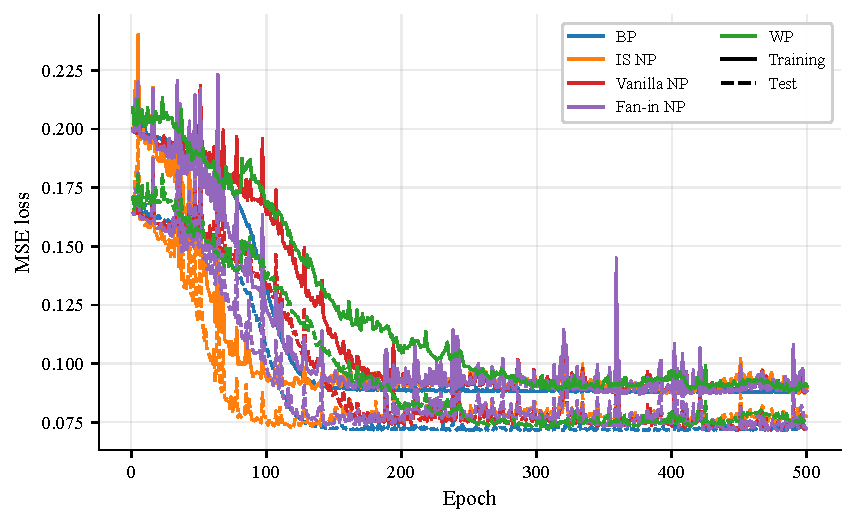
\includegraphics[width=\textwidth]{ResultAssets/figures/sinus_loss.pdf}
        \caption{Training and test loss.}
        \label{fig:sinus_loss}
    \end{subfigure}

    \vspace{0.4cm}

    \begin{subfigure}{0.48\textwidth}
        \centering
        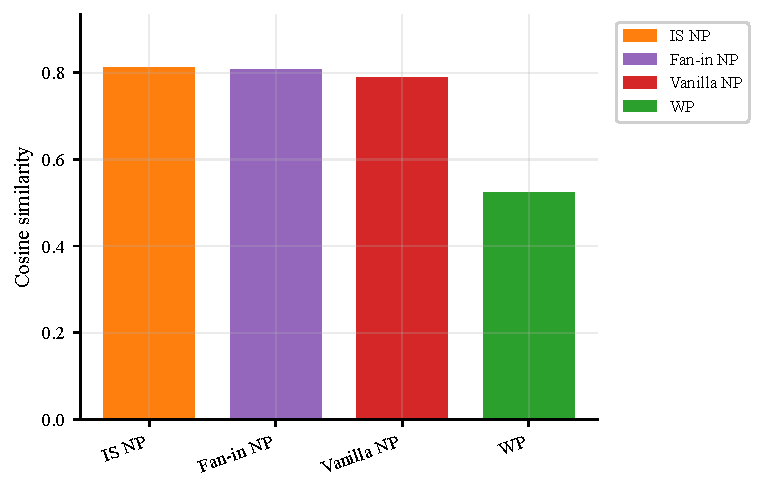
\includegraphics[width=\textwidth]{ResultAssets/figures/sinus_cosine.pdf}
        \caption{Cosine similarity.}
        \label{fig:sinus_cosine}
    \end{subfigure}
    \hfill
    \begin{subfigure}{0.48\textwidth}
        \centering
        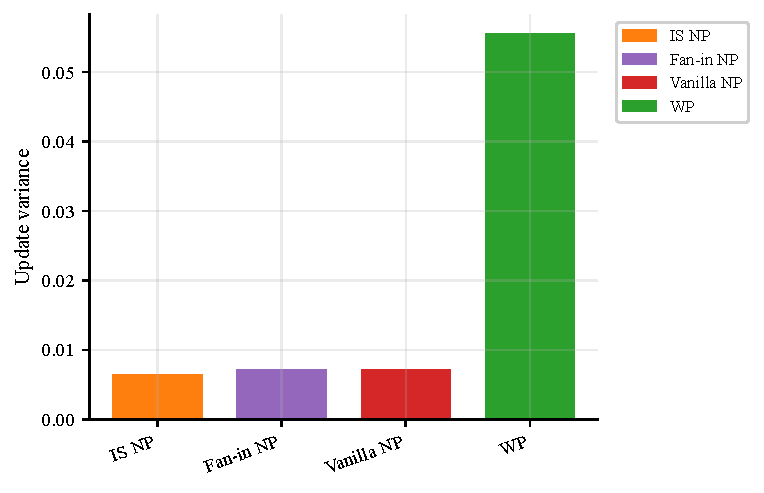
\includegraphics[width=\textwidth]{ResultAssets/figures/sinus_variance.pdf}
        \caption{Estimator variance.}
        \label{fig:sinus_variance}
    \end{subfigure}
    \caption{Results for the sinus regression task.}
    \label{fig:sinus_results}
\end{figure}
\FloatBarrier

\subsection{California Housing Regression}

Backpropagation reaches the lowest training and test loss on the California housing task. It obtains a best test loss of \(0.256\), corresponding to a test \(R^2\) of \(0.741\). Among the perturbation methods, IS-NP obtains the lowest test loss, with \(0.338\) and a test \(R^2\) of \(0.659\). WP follows with a test loss of \(0.345\), vanilla NP reaches \(0.354\), and fan-in NP reaches \(0.390\). WP reaches its convergence criterion earliest among all methods, at epoch \(18\), while IS-NP converges later at epoch \(54\).

The estimator diagnostics show clearer separation between the methods. Vanilla NP has the highest cosine similarity, with \(0.473\), followed closely by IS-NP with \(0.459\). Fan-in NP obtains \(0.368\), while WP is substantially lower at \(0.118\). The variance ranking is different: IS-NP has the lowest estimator variance at \(0.0162\), followed by vanilla NP at \(0.0200\), fan-in NP at \(0.0847\), and WP at \(0.792\). Thus, WP has the weakest estimator diagnostics despite converging quickly in terms of training loss.

For the California housing task, the relationship between estimator diagnostics and final performance is less direct than on the harder classification tasks. IS-NP has the lowest variance and the best final performance among the perturbation methods, while vanilla NP has slightly higher cosine similarity but worse final loss. WP has low cosine similarity and high variance, but still reaches a competitive final loss and the fastest convergence criterion. Overall, the perturbation methods all learn meaningful predictors, but the ranking between them is less clean than on the more complex tasks.

\begin{figure}[!htbp]
    \centering
    \begin{subfigure}{0.95\textwidth}
        \centering
        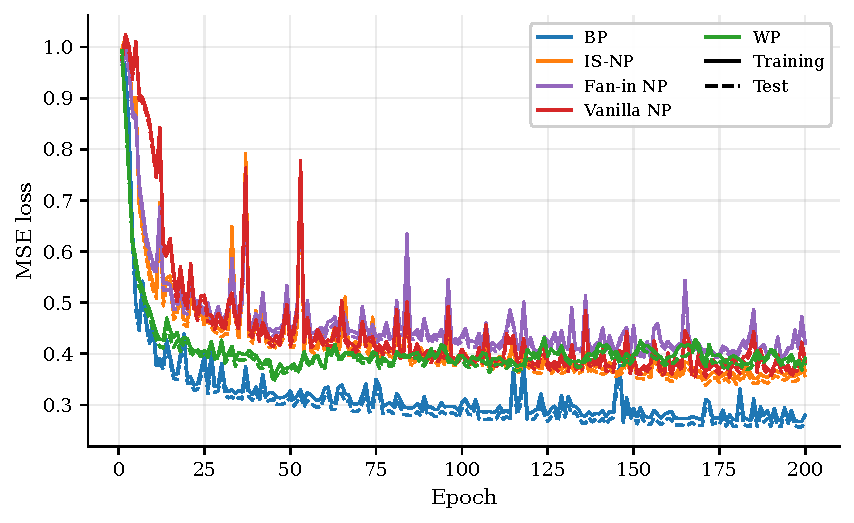
\includegraphics[width=\textwidth]{ResultAssets/figures/california_housing_loss.pdf}
        \caption{Training and test loss.}
        \label{fig:california_housing_loss}
    \end{subfigure}

    \vspace{0.4cm}

    \begin{subfigure}{0.48\textwidth}
        \centering
        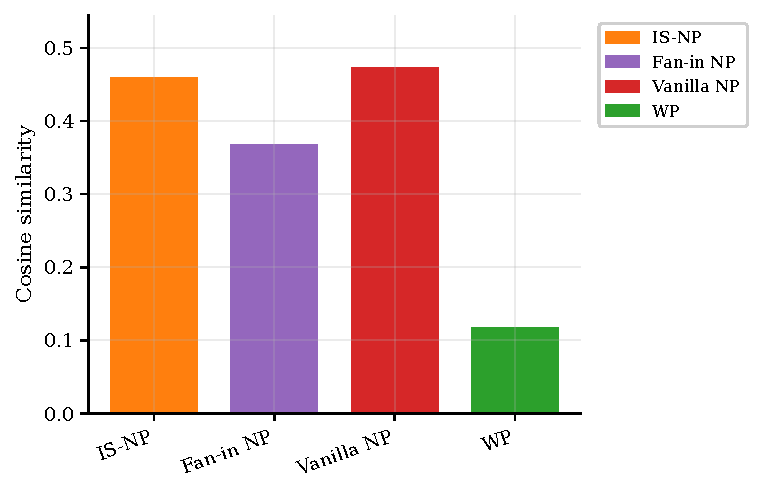
\includegraphics[width=\textwidth]{ResultAssets/figures/california_housing_cosine.pdf}
        \caption{Cosine similarity.}
        \label{fig:california_housing_cosine}
    \end{subfigure}
    \hfill
    \begin{subfigure}{0.48\textwidth}
        \centering
        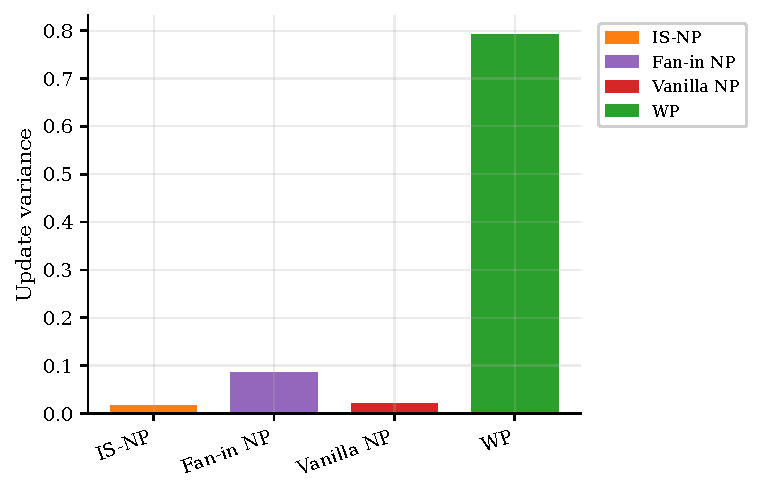
\includegraphics[width=\textwidth]{ResultAssets/figures/california_housing_variance.pdf}
        \caption{Estimator variance.}
        \label{fig:california_housing_variance}
    \end{subfigure}
    \caption{Results for the California housing regression task.}
    \label{fig:california_housing_results}
\end{figure}
\FloatBarrier

\subsection{MNIST Classification}

Backpropagation achieves the best performance on the MNIST classification task, reaching a best test loss of \(0.00588\) and a best test accuracy of \(0.976\). Among the perturbation methods, IS-NP performs best, with a best test loss of \(0.0122\) and a best test accuracy of \(0.949\). Fan-in NP follows with a test loss of \(0.0199\) and accuracy of \(0.917\), while vanilla NP reaches \(0.0270\) and \(0.901\). WP performs worst among the perturbation methods, with a test loss of \(0.0418\) and test accuracy of \(0.810\). IS-NP also converges earlier than the other node perturbation methods, reaching the convergence criterion at epoch \(94\), compared with \(169\) for fan-in NP and \(189\) for vanilla NP.

The estimator diagnostics show a clear separation between WP and the node perturbation methods. IS-NP and fan-in NP have the highest cosine similarities, with \(0.215\) and \(0.210\), respectively. Vanilla NP is lower at \(0.135\), while WP is close to zero at \(0.00973\). The variance results show the same overall pattern. IS-NP has the lowest estimator variance at \(1.18\cdot 10^{-5}\), followed by fan-in NP at \(1.48\cdot 10^{-5}\), vanilla NP at \(4.33\cdot 10^{-5}\), and WP at \(0.00793\).

For MNIST, the relationship between estimator diagnostics and learning performance is clear. The methods with higher cosine similarity and lower estimator variance also obtain better training and test performance. IS-NP has the strongest diagnostics among the perturbation methods and also reaches the best perturbation-based loss and accuracy. WP has the weakest diagnostics and the weakest final performance.

\begin{figure}[!htbp]
    \centering
    \begin{subfigure}{0.48\textwidth}
        \centering
        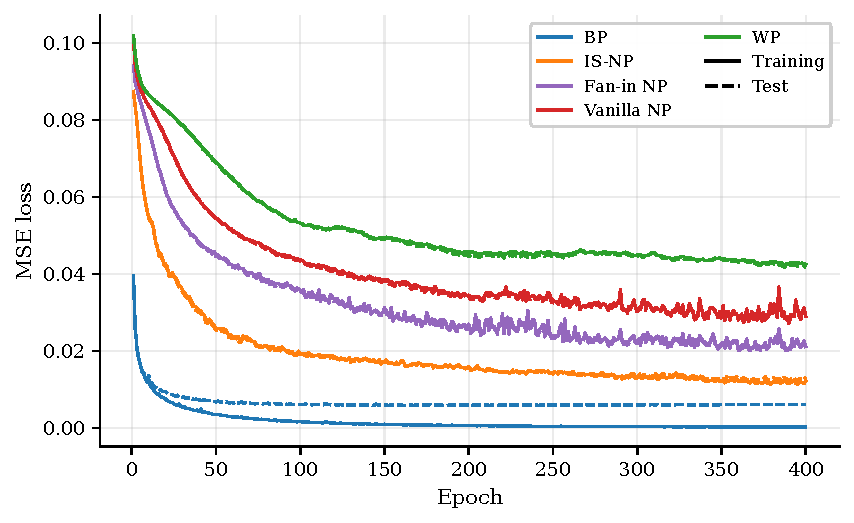
\includegraphics[width=\textwidth]{ResultAssets/figures/mnist_loss.pdf}
        \caption{Training and test loss.}
        \label{fig:mnist_loss}
    \end{subfigure}
    \hfill
    \begin{subfigure}{0.48\textwidth}
        \centering
        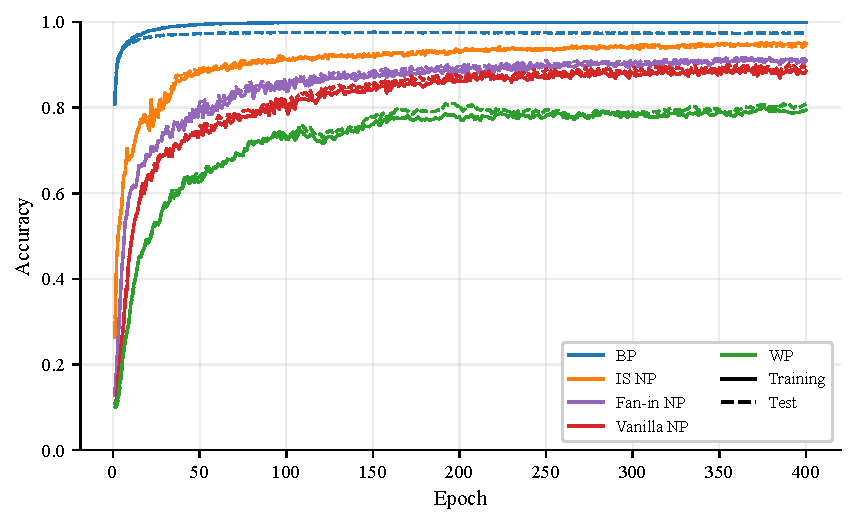
\includegraphics[width=\textwidth]{ResultAssets/figures/mnist_accuracy.pdf}
        \caption{Training and test accuracy.}
        \label{fig:mnist_accuracy}
    \end{subfigure}

    \vspace{0.4cm}

    \begin{subfigure}{0.48\textwidth}
        \centering
        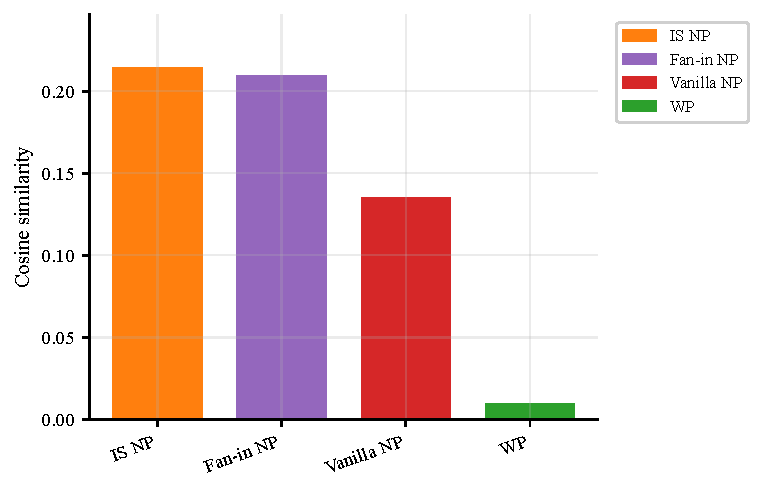
\includegraphics[width=\textwidth]{ResultAssets/figures/mnist_cosine.pdf}
        \caption{Cosine similarity.}
        \label{fig:mnist_cosine}
    \end{subfigure}
    \hfill
    \begin{subfigure}{0.48\textwidth}
        \centering
        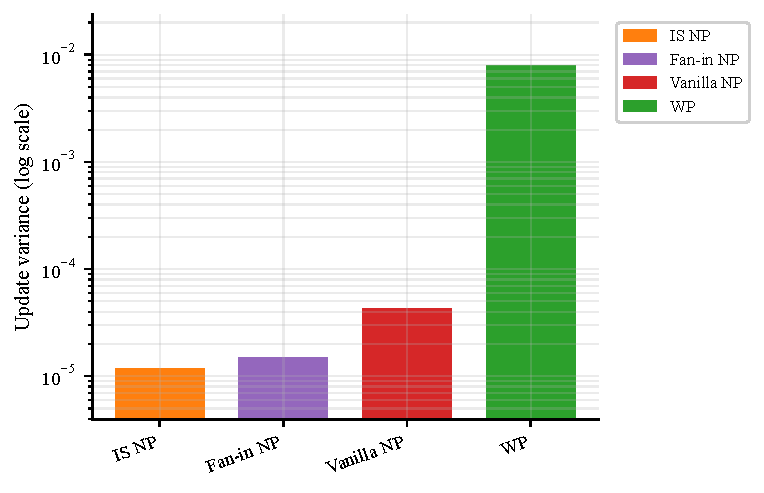
\includegraphics[width=\textwidth]{ResultAssets/figures/mnist_variance.pdf}
        \caption{Estimator variance.}
        \label{fig:mnist_variance}
    \end{subfigure}
    \caption{Results for the MNIST classification task.}
    \label{fig:mnist_results}
\end{figure}
\FloatBarrier

\subsection{CIFAR-10 Classification}

Backpropagation achieves the best performance on the CIFAR-10 classification task, reaching a best test loss of \(0.0678\) and a best test accuracy of \(0.499\). The perturbation methods reduce the loss, but plateau at substantially worse values. Among the perturbation methods, IS-NP performs best, with a best test loss of \(0.0806\) and a best test accuracy of \(0.339\). Fan-in NP follows with a test loss of \(0.0820\) and accuracy of \(0.321\), while vanilla NP reaches \(0.0832\) and \(0.296\). WP performs worst, with a test loss of \(0.0851\) and test accuracy of \(0.264\).

The estimator diagnostics show the same ordering as the learning curves. IS-NP has the highest cosine similarity among the perturbation methods, with \(0.0483\), followed by fan-in NP at \(0.0436\), vanilla NP at \(0.0260\), and WP at \(9.92\cdot 10^{-4}\). The variance results also separate WP clearly from the node perturbation methods. IS-NP has the lowest variance at \(1.22\cdot 10^{-5}\), followed by fan-in NP at \(1.31\cdot 10^{-5}\), vanilla NP at \(3.65\cdot 10^{-5}\), and WP at \(0.0355\).

For CIFAR-10, the relationship between estimator diagnostics and learning performance is clear. The methods with higher cosine similarity and lower estimator variance also reach better training and test performance. Compared with the simpler tasks, the differences between perturbation methods are more visible, and the gap between all perturbation methods and backpropagation is substantially larger.

\begin{figure}[!htbp]
    \centering
    \begin{subfigure}{0.48\textwidth}
        \centering
        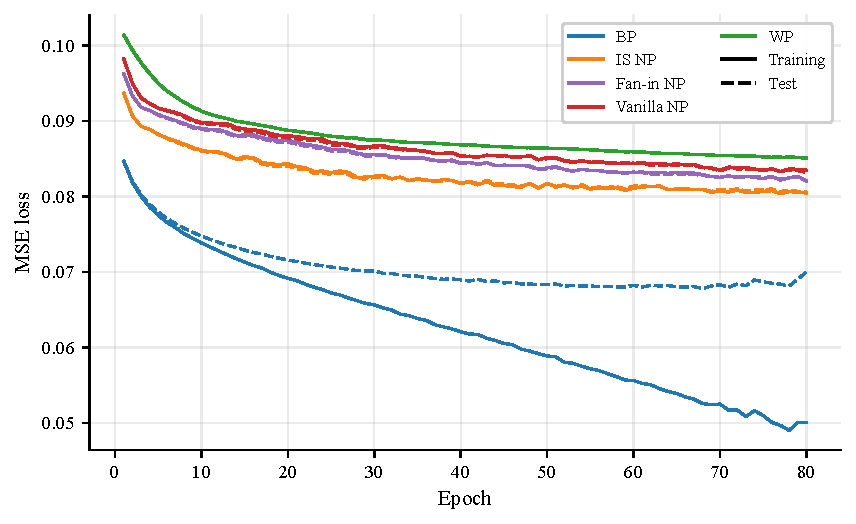
\includegraphics[width=\textwidth]{ResultAssets/figures/cifar10_loss.pdf}
        \caption{Training and test loss.}
        \label{fig:cifar10_loss}
    \end{subfigure}
    \hfill
    \begin{subfigure}{0.48\textwidth}
        \centering
        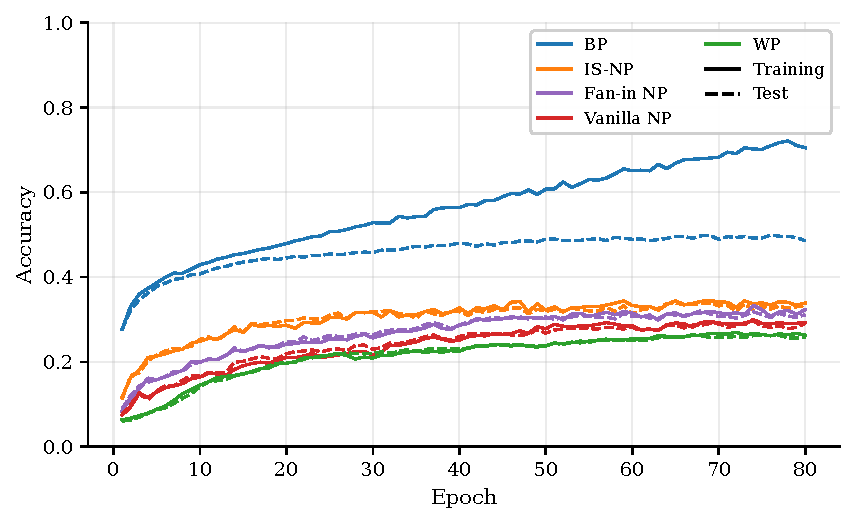
\includegraphics[width=\textwidth]{ResultAssets/figures/cifar10_accuracy.pdf}
        \caption{Training and test accuracy.}
        \label{fig:cifar10_accuracy}
    \end{subfigure}

    \vspace{0.4cm}

    \begin{subfigure}{0.48\textwidth}
        \centering
        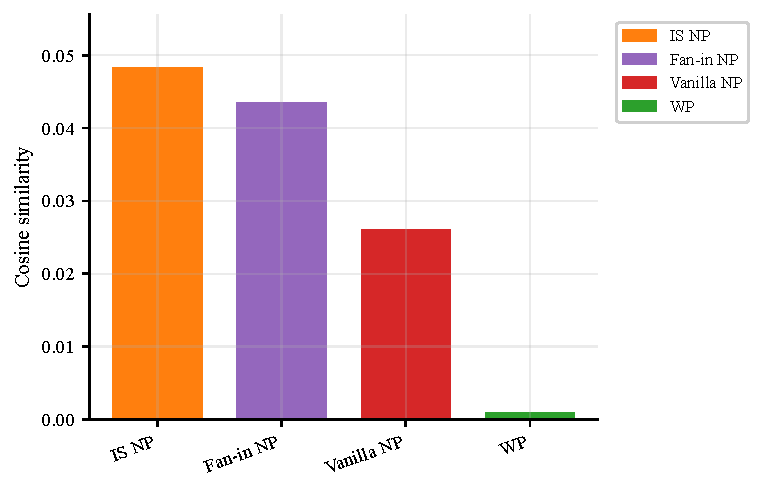
\includegraphics[width=\textwidth]{ResultAssets/figures/cifar10_cosine.pdf}
        \caption{Cosine similarity.}
        \label{fig:cifar10_cosine}
    \end{subfigure}
    \hfill
    \begin{subfigure}{0.48\textwidth}
        \centering
        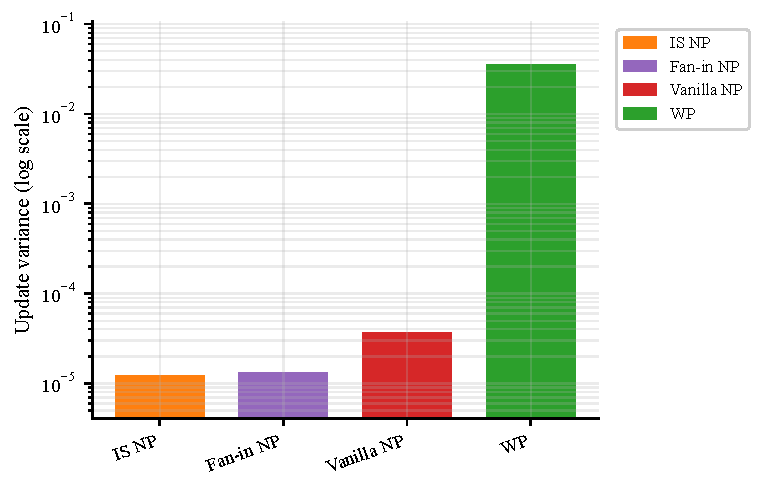
\includegraphics[width=\textwidth]{ResultAssets/figures/cifar10_variance.pdf}
        \caption{Estimator variance.}
        \label{fig:cifar10_variance}
    \end{subfigure}
    \caption{Results for the CIFAR-10 classification task.}
    \label{fig:cifar10_results}
\end{figure}
\FloatBarrier

\subsection{Scaled Input Sensitivity}

Scaling the sinus input range from \([-1,1]\) to \([-5,5]\) changes the estimator diagnostics differently across methods. IS-NP and WP are only weakly affected by the input scaling, while vanilla NP and fan-in NP degrade substantially. For vanilla NP and fan-in NP, cosine similarity decreases clearly under the scaled input setting, whereas IS-NP remains close to its original level and WP changes comparatively little. The same pattern appears in estimator variance: vanilla NP and fan-in NP show a large increase in variance, while IS-NP and WP remain comparatively stable.

The scaled-input experiment therefore separates the methods more clearly than the original sinus regression task. In the default \([-1,1]\) setting, all node perturbation methods have relatively high cosine similarity and low estimator variance. Under input scaling, the diagnostics for vanilla NP and fan-in NP worsen, while IS-NP remains the strongest node perturbation method. This result is consistent across both diagnostic metrics shown in Figure~\ref{fig:scaled_input_results}: the methods that account for the actual effect of input scale, WP and IS-NP, are less sensitive to the change than methods using fixed or layer-width-based node perturbation scales.

\begin{figure}[!htbp]
    \centering
    \begin{subfigure}{0.48\textwidth}
        \centering
        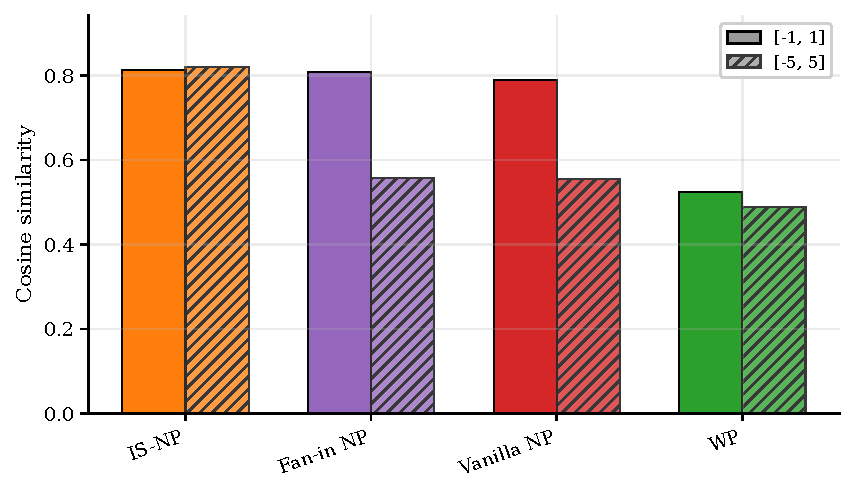
\includegraphics[width=\textwidth]{ResultAssets/figures/sinus_scaled_input_cosine_comparison.pdf}
        \caption{Cosine similarity.}
        \label{fig:sinus_scaled_input_cosine}
    \end{subfigure}
    \hfill
    \begin{subfigure}{0.48\textwidth}
        \centering
        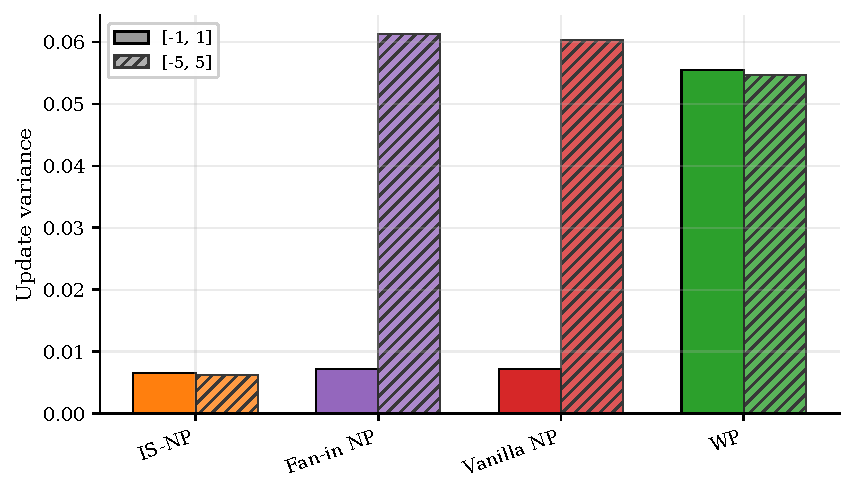
\includegraphics[width=\textwidth]{ResultAssets/figures/sinus_scaled_input_variance_comparison.pdf}
        \caption{Estimator variance.}
        \label{fig:sinus_scaled_input_variance}
    \end{subfigure}
    \caption{Effect of scaling the sinus input range from $[-1, 1]$ to $[-5, 5]$.}
    \label{fig:scaled_input_results}
\end{figure}
\FloatBarrier

\begin{sidewaystable}[!p]
    \centering
    \scriptsize
    \caption{Summary of training performance, estimator alignment, estimator variance, and convergence speed.}
    \label{tab:results_summary}
    \input{ResultAssets/tables/results_summary.tex}
\end{sidewaystable}
\FloatBarrier
